%
\begin{align}
    Y = X^2 + 3\\
\implies     X = \sqrt{Y - 3}
\end{align}
Substituting $k = \sqrt{y-3}$ in \eqref{poisson/1/eq:1},
\begin{align}
p_Y(y) = 
    \begin{cases} 
      \frac{e^{-\lambda}\lambda^{\sqrt{y-3}}}{\sqrt{\brak{y-3}}!}, & y=3,4,7,12,...\\
      0&\text{otherwise}
   \end{cases}
\end{align}
Hence, the correct option is \brak{A}.
\begin{figure}[hb]
    \centering
    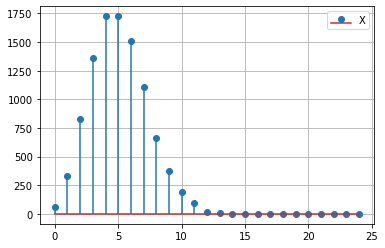
\includegraphics[width=\columnwidth]{poisson/solutions/1/Figures/FigureX.png}
    \caption{Poisson stem plot for X \brak{\lambda = 5}}
    \label{poisson/1/fig:plot1}
\end{figure}
\begin{figure}[hb]
    \centering
    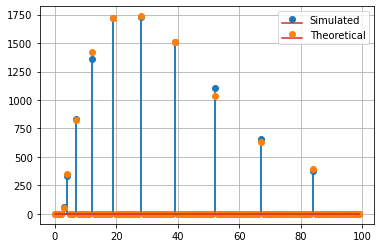
\includegraphics[width=\columnwidth]{poisson/solutions/1/Figures/FigureComp.png}
    \caption{Stem plot for Y (Simulated and Theoretical) \brak{\lambda = 5}}
    \label{poisson/1/fig:plot3}
\end{figure}
